\documentclass{article}
\usepackage{ctex}
\title{大物作业}
\author{张博涵-应化1903(学号:1912020312)}
\date{\today}
\usepackage{graphics} 
\usepackage{listings}
\usepackage{framed}
\usepackage{amsthm,amsmath,amssymb}
\usepackage{wrapfig}
\usepackage{graphicx}
\usepackage{mathrsfs}
\bibliographystyle{plain}
\usepackage{subfiles}
\usepackage{listings}
\usepackage{booktabs}
\usepackage{graphicx,times}
\usepackage{subfigure}         
\usepackage{natbib}
\usepackage{amssymb,amsmath}
\usepackage{url}
\usepackage{geometry}
\usepackage{xcolor}
\usepackage{setspace}
\usepackage{subfigure}
\usepackage{tikz}
\everymath{\displaystyle}
\usepackage{booktabs}
\usepackage{array}
\begin{document}
\maketitle

\textbf{题1-32}
由题构造如图所示 Gauss 面:
\begin{figure}[h]
	\centering
	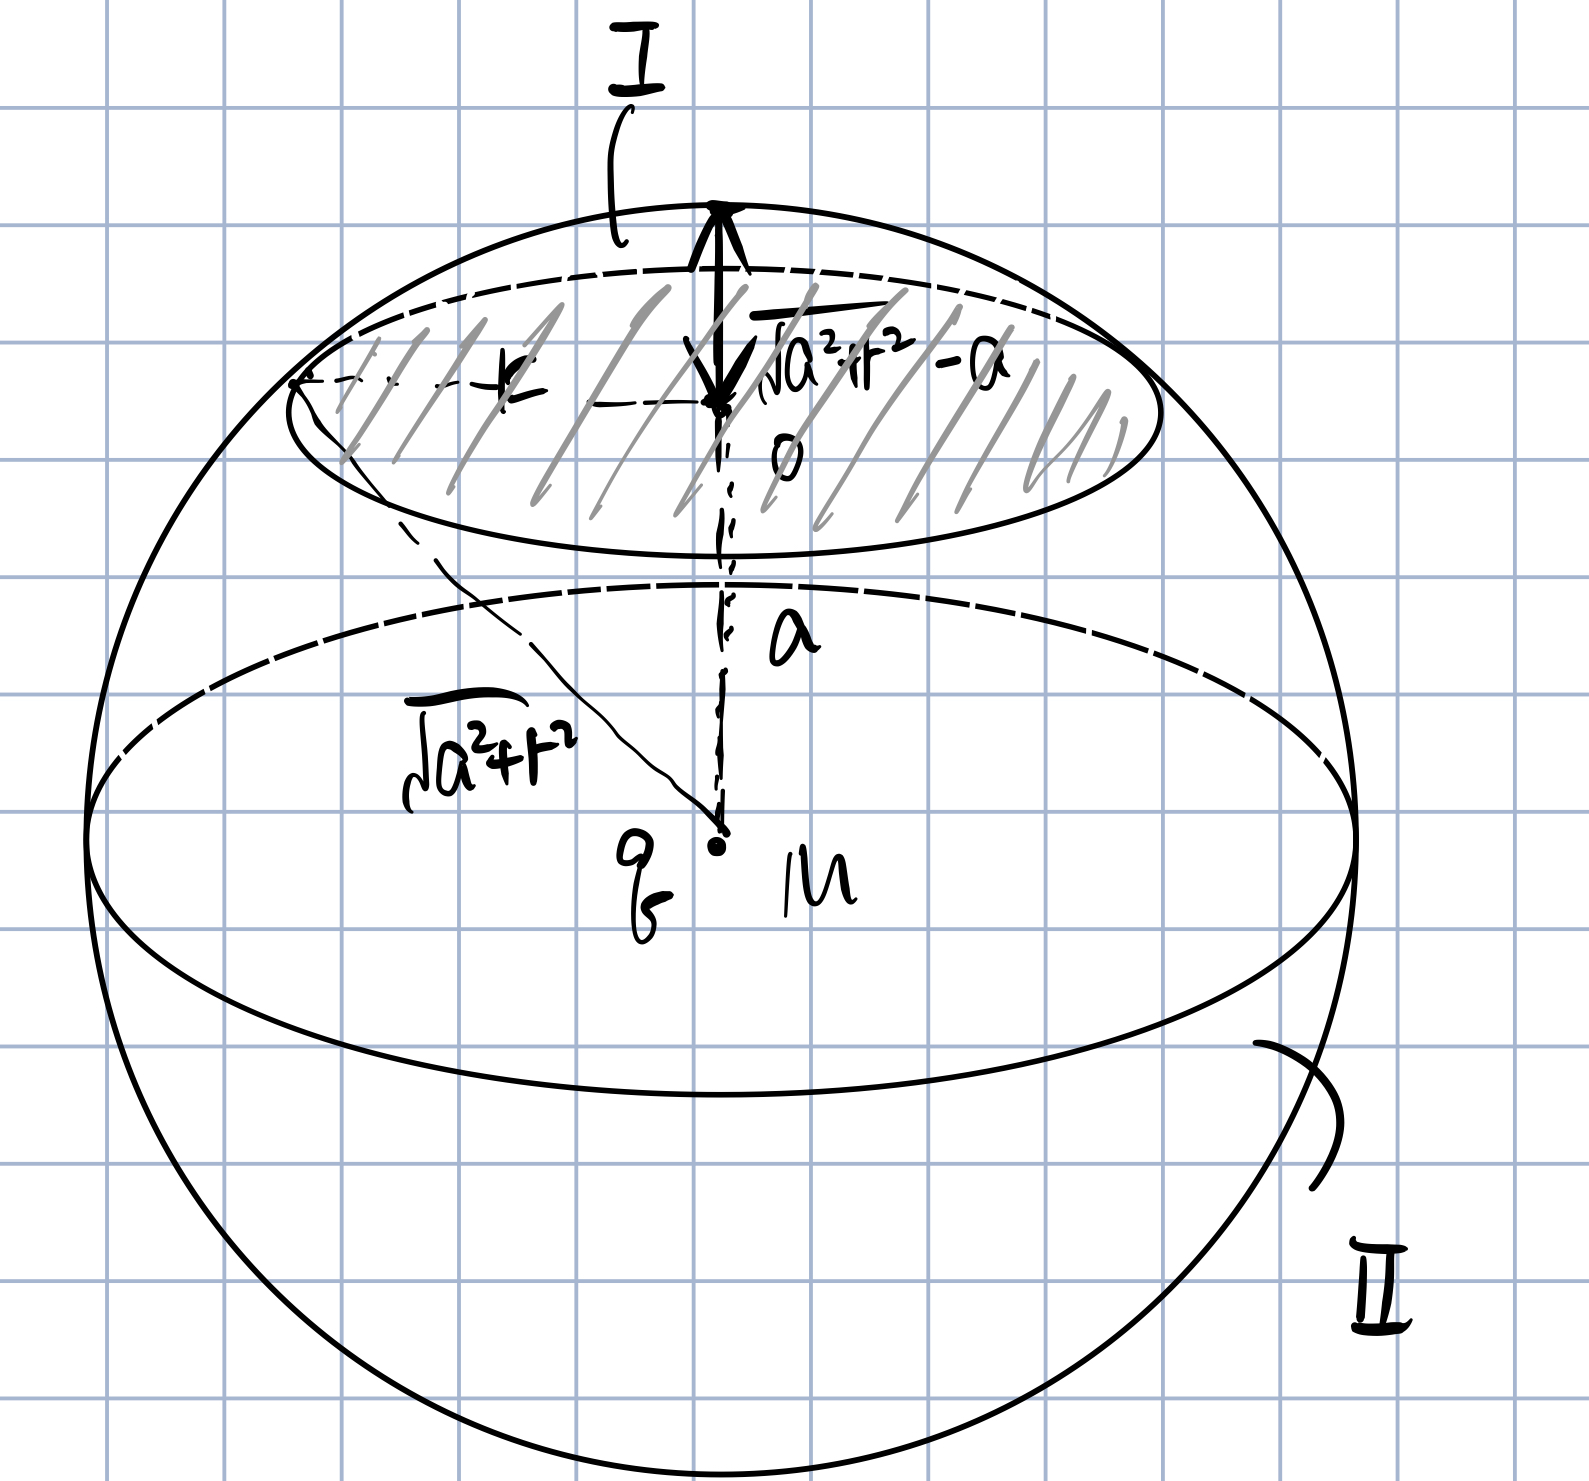
\includegraphics[scale = 0.1]{1}
	\caption{题1-32}
\end{figure}


以所给圆盘为一球的切面,以 M 点为圆心作球面,并定义以所给圆盘为底的球冠为曲面\uppercase\expandafter{\romannumeral1},整个球面除去这一部分为曲面\uppercase\expandafter{\romannumeral2}。

利用电场Gauss定理,可以知道$\displaystyle\Phi _{\uppercase\expandafter{\romannumeral1}+\uppercase\expandafter{\romannumeral2}} =\dfrac{q}{\varepsilon_0}$

分析这个以 M 点为球心的球面的对称性,可以发现,球面上任何一点的电场强度大小是一致的,并且此时面的法向法向和电场强度方向共线,取球面外侧为正向,则两个面之比的电通量与两个面积之比相等,即有比例关系:
\begin{equation}
	\dfrac{\Phi _{\uppercase\expandafter{\romannumeral1}}}{\Phi _{\uppercase\expandafter{\romannumeral1}+\uppercase\expandafter{\romannumeral2}}} = \dfrac{\Phi _{\uppercase\expandafter{\romannumeral1}}}{\dfrac{q}{\varepsilon_0}} = \dfrac{S_{\uppercase\expandafter{\romannumeral1}}}{S_{\uppercase\expandafter{\romannumeral1}+\uppercase\expandafter{\romannumeral2}}}
\end{equation}
其中$S_{\uppercase\expandafter{\romannumeral1}}$、$S_{\uppercase\expandafter{\romannumeral1}+\uppercase\expandafter{\romannumeral2}}$分别表示球冠和球壳 的面积


根据图中所示,有比例关系:
\begin{equation}
	\dfrac{S_{\uppercase\expandafter{\romannumeral1}}}{S_{\uppercase\expandafter{\romannumeral1}+\uppercase\expandafter{\romannumeral2}}} = \dfrac{2\pi \sqrt{a
	^2+r^2}(\sqrt{a^2+r^2}-a)}{4\pi (a^2 + r^2)}
\end{equation}

这样就可以解得:
\begin{equation}
	\Phi _{\uppercase\expandafter{\romannumeral1}} = \dfrac{2\pi q\sqrt{a
	^2+r^2}(\sqrt{a^2+r^2}-a)}{4\pi \varepsilon_0(a^2 + r^2)}
	=\dfrac{q\sqrt{a^2+r^2}(\sqrt{a^2+r^2}-a)}{2\varepsilon_0(a^2 + r^2)}
\end{equation}
取球冠和圆盘所构成的闭曲面,穿入的电通要等于穿出的电通,所以穿过圆盘的电通量也为$\Phi _{\uppercase\expandafter{\romannumeral1}}$即$\dfrac{q\sqrt{a^2+r^2}(\sqrt{a^2+r^2}-a)}{2\varepsilon_0(a^2 + r^2)}$。\\



\textbf{题1-42}取半径$r\in [R_1,R_2]$取半径微小增量$dr$在这微小扇形上带有电荷量为$dq$,则有以下关系:
\begin{equation}
		dq = \sigma \theta_0 r dr 
\end{equation}
则这部分在原点所激发的电场产生的电势为$du=\dfrac{1}{4\pi \varepsilon_0}\dfrac{dq}{r} $

则经过一次积分可得整个扇形带电区域在原点产生的电场为:
\begin{equation}
	U = \int_{R_1}^{R_2}du = \dfrac{1}{4\pi \varepsilon_0}\int_{R_1}^{R_2}\dfrac{ \sigma \theta_0 r dr }{r} =\dfrac{\sigma \theta_0}{4\pi \varepsilon_0}\int_{R_1}^{R_2}dr=\dfrac{\sigma \theta_0}{4\pi \varepsilon_0}(R_2-R_1)
\end{equation}
	
\end{document}
